\documentclass{article}

\usepackage{hyperref}
\usepackage{gensymb}
\usepackage{enumitem}
\usepackage{amssymb}
\usepackage{wrapfig}
\usepackage{subfigure}
\usepackage{braket}
\usepackage{amsmath}
\usepackage{graphicx}
\usepackage{mathtools}
\usepackage[letterpaper, margin=1in]{geometry}
\setlength{\parindent}{0cm}

\title{Pointing Calibration}
\author{Tritium $(e,e'p)$ Experiment\\Efrain Segarra}
\begin{document}

\maketitle


%%%%%%%%%%%%%%%%%%%%%%%%%%%%%%%%%%%%%%%%%%%%%%%%%%%%%%%%%%%%%%%%%%%%%%%%%%%%%%%%%%%%%%%%%
\section*{Procedure}
The goal is to calibrate the central spectrometer angles at each kinematics in order to have optimal reconstructions.\\

Since we did not take a survey at mid or fast kinematics, only at slow, we have to work a bit harder to get the pointing calibration done, but it is possible since we did take a run with a multi-foil target (ideally we'd want the single foil target, but this will work) at each kinematics. We also do not have a measurement of the target location with respect to the hall center -- we should make sure this is finalized before the run is over. The best case scenario would have been to take survey and have single carbon foil data at each kinematics. But we'll deal!\\

The first step is to find the $z_{tr}$ (the position of the middle foil with respect to the hall center $(0,0,0)$ coordinates) since there is currently an ambiguous target survey.\\

This can be done by going to the kinematics where we do have a survey (slow) and measurements on multi-foil target. The multi-foil target looks like it has 11 scattering centers, and I assume that the middle foil was intentioned to be positioned to be at $(0,0,0)$ -- and this is the foil to find $z_{tr}$ on.\\

With this distribution of $y_{tr}$, and a distribution for the beam position in $x$, I can extract $z_{tr}$. Of course, the $y$ position of the beam will not change $z_{tr}$ in the $z-x$ plane. Not doing a calculation event-by-event, but instead, averaging over all events, we can estimate $z_{tr}$ by:
\begin{equation*}
	\begin{gathered}
		z_{tr} \sin{\theta_c} = -y_{tr} - \delta + x_\textrm{beam} \cos{\theta_c} \textrm{     for LHRS} \\
		z_{tr} \sin{\theta_c} = y_{tr} + \delta - x_\textrm{beam} \cos{\theta_c} \textrm{     for RHRS} \\
	\end{gathered}
\end{equation*}
Where $\delta$ is the mispointing, $\theta_c$ is the spectrometer central angle, related to the vernier angle through $\delta$ -- all given in a typical survey.\\

At some point I hope to add a diagram showing this, but after working with Barak for a while, we`re convinced this is correct. Basically remember that increasing $y_{tr}$ for the LHRS is towards negative $z_{react}$, and for the RHRS, it`s positive. Furthermore, increasing $x_\textrm{beam}$ means increasing $y_{tr}$ for LHRS and RHRS. I also assume that the spectrometer central angles are always positive and $\delta$ positive.\\

Then all that remains is to extract $z_{tr}$ based on the values in the survey and the mean-values of $y_{tr} , x_\textrm{beam}$ for the middle foil, see plots below. Of course a target survey will tell you what $z_{tr}$, so this will serve as a cross check. I remark that this is an average over all events. If one wants to do an event-by-event calculation, then the formulae should be modified slightly to:
\begin{equation*}
	\begin{gathered}
		z_{tr} = -(y_{tr} + \delta) \frac{\cos{(\arctan{\phi_{tr})}}}{\sin{(\theta_c+\arctan{\phi_{tr})}}} + x_\textrm{beam} \cos{(\theta_c + \arctan{\phi_{tr})}}  \textrm{           for LHRS}\\
	\end{gathered}
\end{equation*}
Where $\theta_c = \theta_n + \delta/L$, $\theta_n$ is the angle given by the vernier, and $L = 8.458$ m.\\

\begin{center}
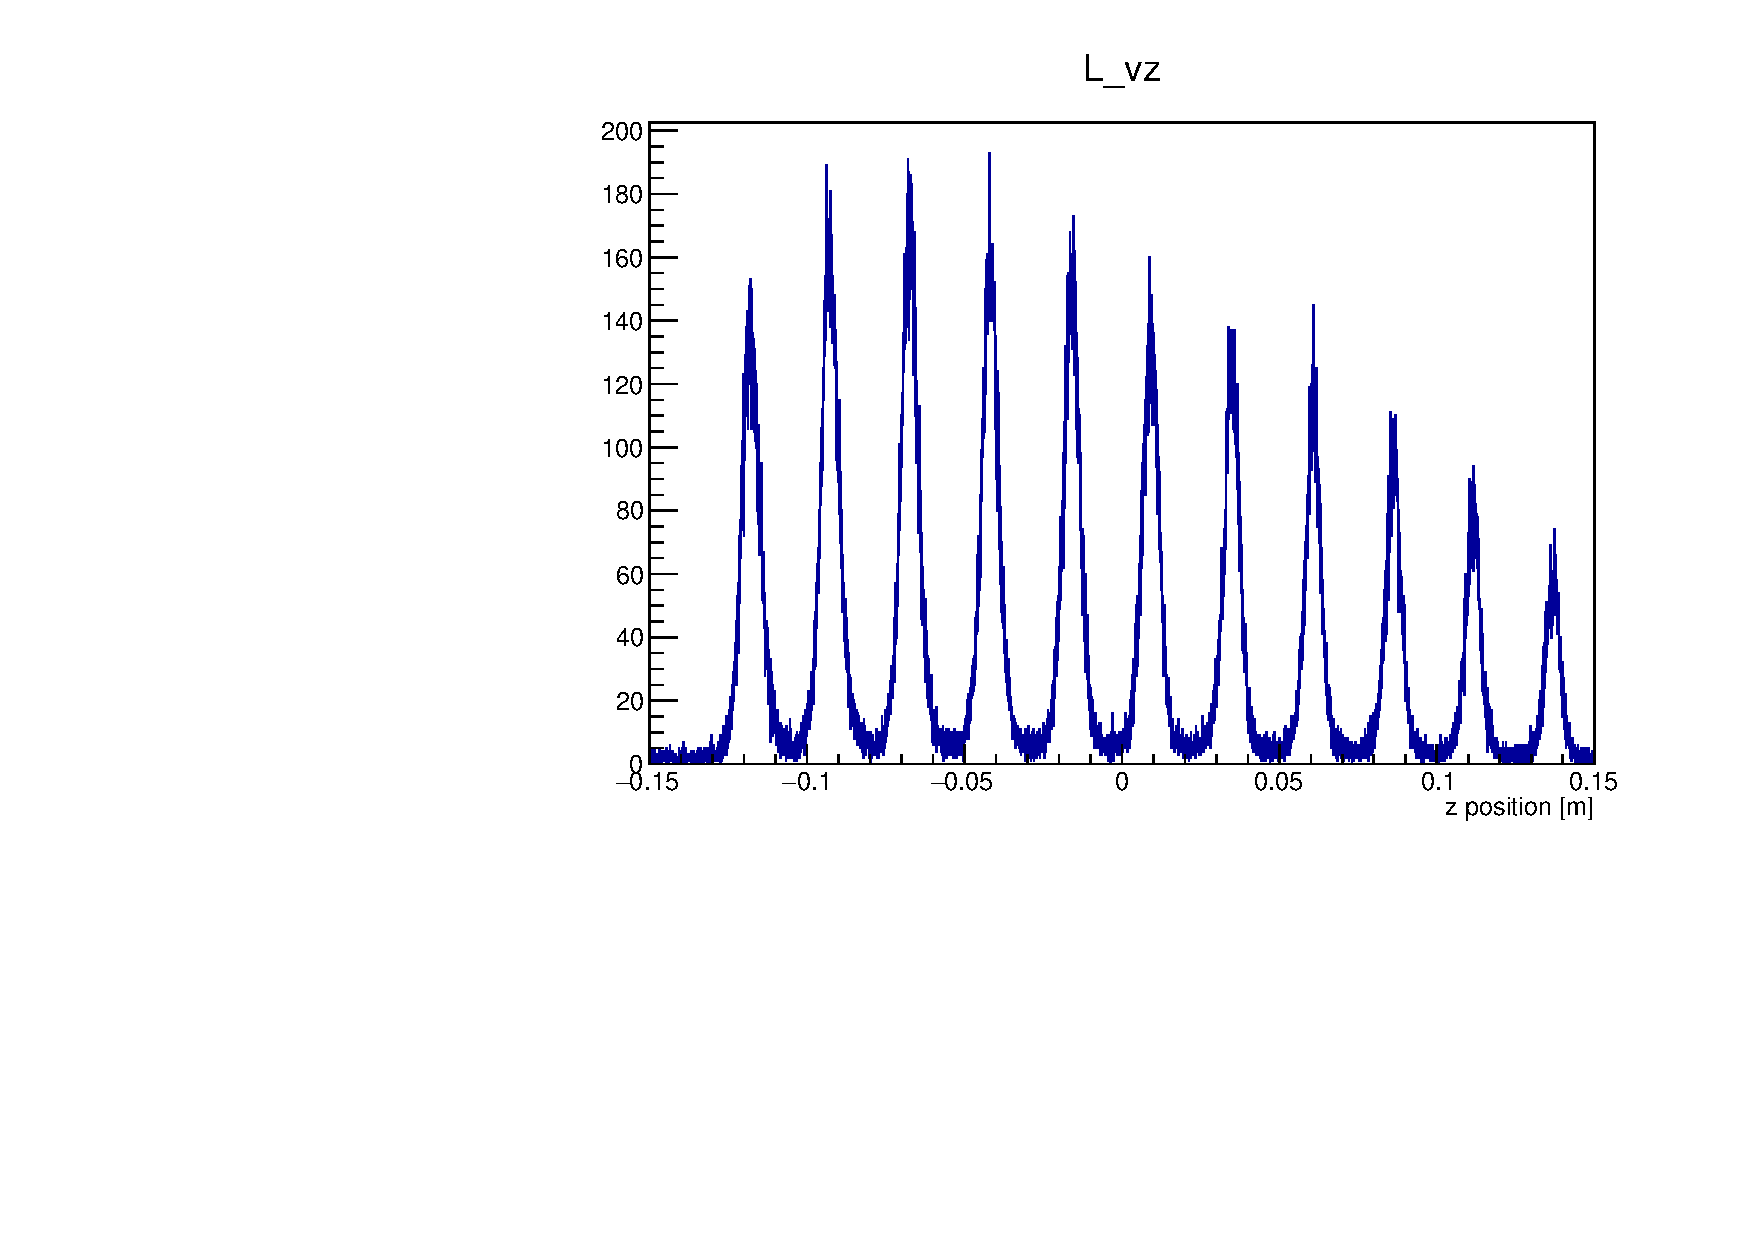
\includegraphics[width=10cm]{zPos.pdf}\\
Vertex reconstructed on LHRS. Here is where I place a cut on the assumed middle foil, and then look at $y_{tr}, x_\textrm{beam}$ distributions to get an average value to extract $z_{tr}$, the offset of this middle foil. I can repeat the same procedure for the RHRS, and check to see if the two results are consistent.
\end{center}

\begin{center}
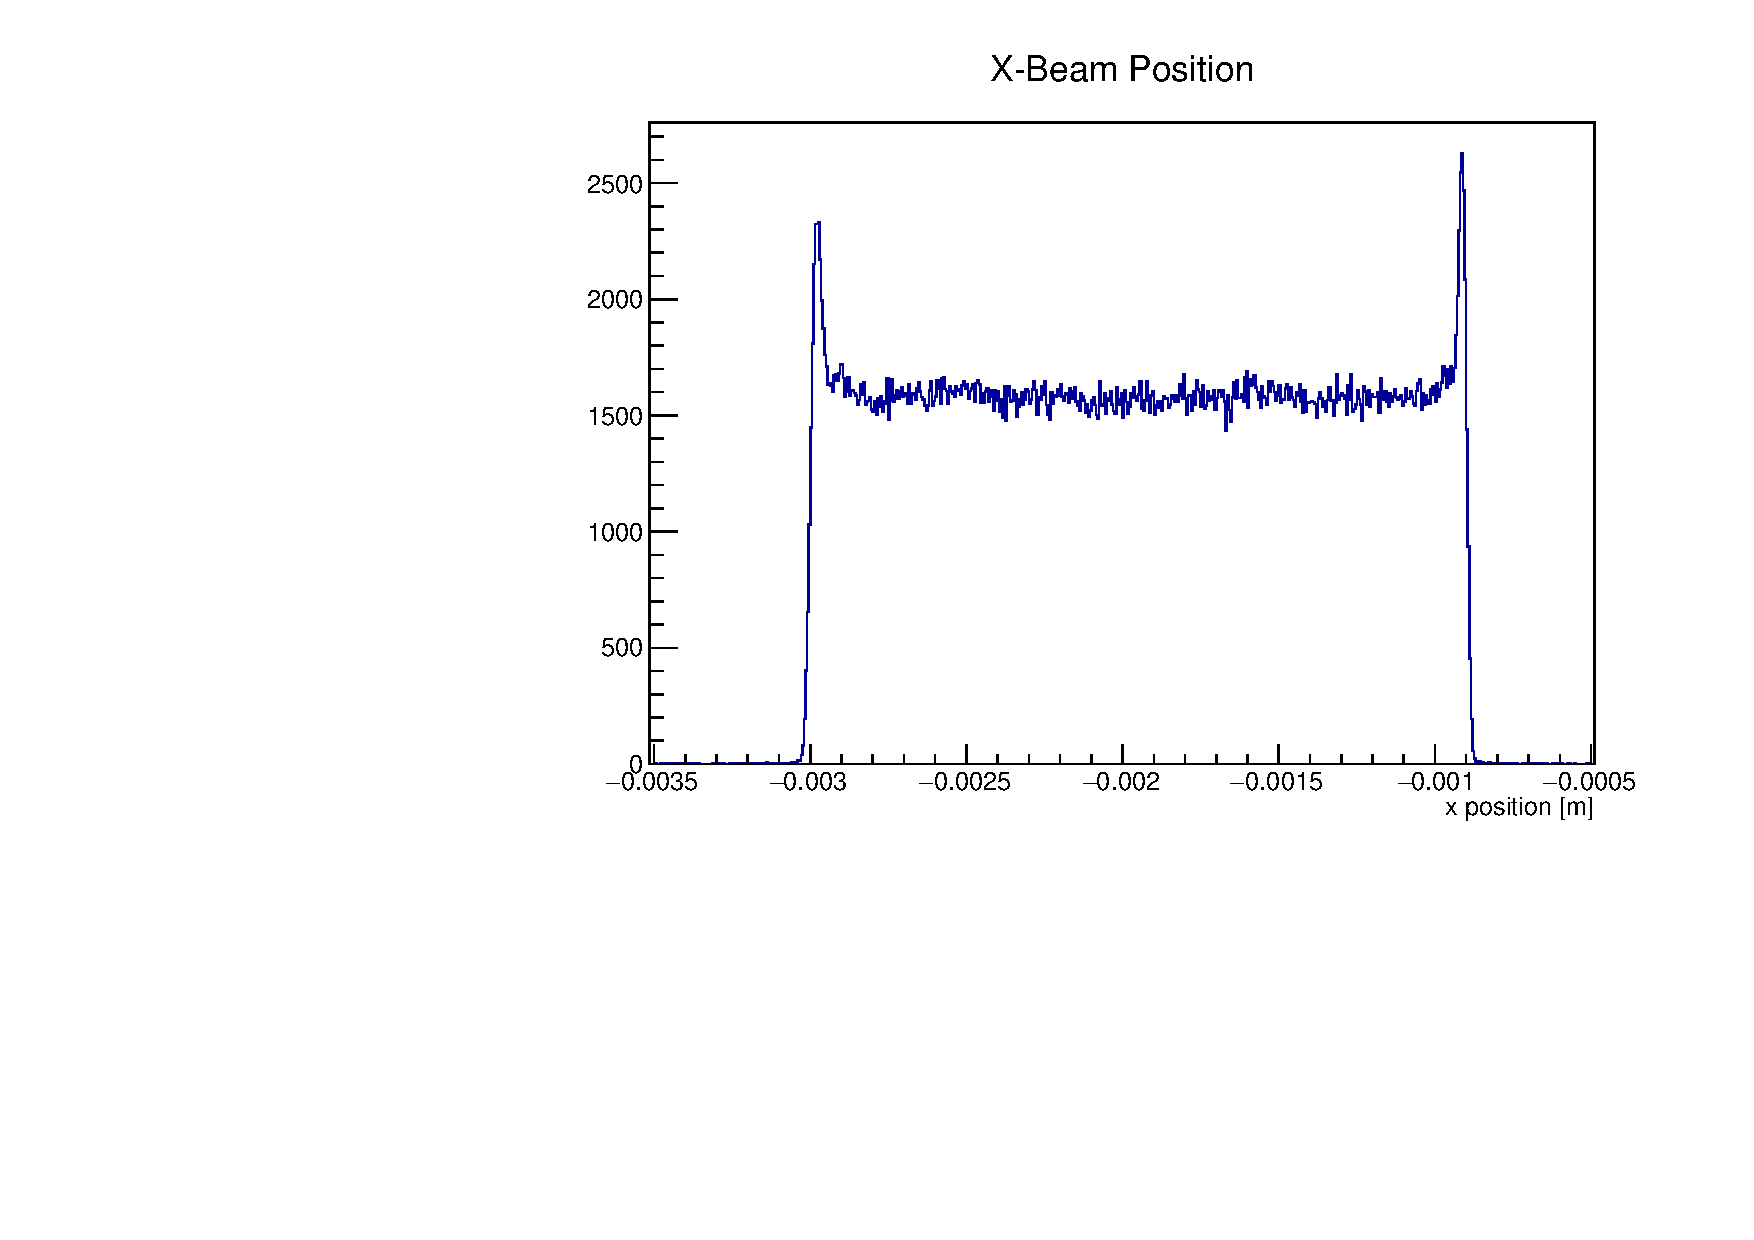
\includegraphics[width=10cm]{beamPos.pdf}\\
\end{center}


So in principle, if we don't have a survey for one kinematical settings, but we know $z_{tr}$, one can calculate $\delta$ (since we know $\theta_n$) on an event-by-event basis, doing some $\chi^2$ minimization, or taking an average of all events and solving numerically for $\delta$. \\

In summary, how I will proceed:
\begin{itemize}
\item{Calculate $z_{tr}$ for a kinematical setting where we have a survey, and thus know $\delta$. I am doing so because for the moment, we do not have a target survey to tell us $z_{tr}$ for the multi-foil runs.}
\item{Using $z_{tr}$, calculate $\delta$ for kinematical settings where we do not have a survey, but do have multi-foil runs, using an averaged method.}
\item{Repeat both using event-by-event processing, and cross-check result.}
\end{itemize}

\clearpage

\section*{Results}
\subsection*{Extracting $z_{tr}$}
Already starting off, I realized there is an inconsistency between what central angle the analyzer assumes, and the vernier angle that the survey quotes (which should be the same). That means the exact solution should be to re-analyze the multi-foil runs in the slow kinematics. Otherwise, the distributions that I use to extract $z_{tr}$, assuming a mispointing $\delta$ from the survey, will be a mispointing on an inconsistent $\theta_n$. The difference between the angles that the analyzer uses, and the survey assumes, is 0.024 mrad and 0.035 mrad (probably below the sensitivity of a survey, but ideally I should re-analyze the file with the same $\theta_n$ assumed.


Starting with first point, taking our slow kinematics, multifoil data, I extract that $z_{tr}$ is $3.309$ mm for the LHRS and $2.915$ mm for the RHRS. These are roughly consistent, but a good cross-check will be the target alignment survey, and to re-analyze the file with the angles that the survey assumed. This of course was doing with the averaging method, so another good cross-check would be to do an event-by-event calculation.\\

This can also be improved, as I did not apply any other cuts to clean the sample, other than a single track in the LHRS (RHRS) to get the $z_{tr}$ estimated from the LHRS (RHRS).\\

Now of course the idea is to use this average $z_{tr}$ to calculate $\delta$ in the kinematics where we did not do a survey -- but did take multi-foil target data -- and correctly point the spectrometers.\\

\subsection*{Extracting $\delta$ for mid kinematics}
Proceeding in the mid kinematics, for the LHRS, with $z_{tr}$ we can now extract the mispointing $\delta$,
\begin{equation*}
	\begin{gathered}
		\textrm{LHRS:       }0 = z_{tr} \sin{\left(\theta_n + \frac{\delta}{L}\right)} + y_{tr} - x_\textrm{beam} \cos{\left(\theta_n + \frac{\delta}{L}\right) } + \delta\\
		\textrm{RHRS:       }0 = z_{tr} \sin{\left(\theta_n + \frac{\delta}{L}\right)} - y_{tr} + x_\textrm{beam} \cos{\left(\theta_n + \frac{\delta}{L}\right) } - \delta\\
	\end{gathered}
\end{equation*}

Using now our multi-foil target, cutting on the middle foil as before, and getting an average $y_{tr}, x_\textrm{beam}$, we can numerically solve for $\delta$ knowing $\theta_n$ (given by the vernier), and $z_{tr}$, extracted above (or ideally with a target alignment survey).\\

With this, I extract a mispointing $\delta=2.179$ mm for mid-kinematics, causing $\theta_c = \theta_n + \delta/L = 17.8017\degree + \delta/L = 17.8165\degree$, a change of 0.258 mrad for the LHRS.\\

Repeating for the RHRS, I extract a mispointing of $\delta=1.225$ mm,  causing $\theta_c = \theta_n + \delta/L = 48.82\degree + \delta/L = 48.8283\degree$, a change of 0.145 mrad for the RHRS.\\

These are in agreement with the order-of-magnitude offsets expected from a survey.


\subsection*{Looking at H(e,e'p) in mid kinematics with pointing correction}
Using these pointing offsets, I now look at the H(e,e'p) data set, and reconstruct the beam energy to see how far off it is from independent measure, that should be accurate to the level of $5\cdot10^{-4}$. The conclusion is that it seems I became about 5.8 MeV more accurate, but still off from 0. In order to see if the mispointing has an effect in other distributions, the files need to be replayed with the updated angles (to allow one to look at the most accurate variables which use extended-target-rastered-beam corrections).\\

This could be still off from 0 for a number of reasons: (1) beam energy not known well enough, (2) errors in ($y'_{\textrm{tar}},x'_{\textrm{tar}}$) not calibrated, (3) non-optimized algorithm to extract $z_{tr},\delta$.

\subsection*{Next Steps}
\begin{itemize}
\item{Re-replay the multi-foil runs in slow kinematics to make the central angle consistent with the survey central angle, so if one uses their $\delta$, it's off the same central angle.}
\item{Improve extraction of $z_{tr}$ for the middle foil instead of doing average calculation -- such as an event-by-event?}
\item{Improve extraction of $\delta$, again by doing event-by-event.}
\item{Calibrate beam energy to a level below $10^{-4}$}
\item{Calibrate optics ($y'_{\textrm{tar}},x'_{\textrm{tar}}$) with sieve data (LHRS has optics data in late March from Marathon -- need to check angles)}
\item{Using the single carbon foil data took on slow kinematics (where there is the survey) to cross check target-alignment}
\item{Understanding target alignment survey (talk with Dave Meekins)}
\item{After optimizing the best $\delta$ for mid kinematics, re-analyze the files with the corrected central angle in order to look at extended-target-rastered-beam corrected variables}
\end{itemize}


\subsection*{H(e,e'p) Distributions with Pointing Corrections}
With the pointing corrections, one really should re-analyze the file with updated central angles in order to look at the most accurate kinematic variables that include extended-target-rastered-beam corrections. However, what I can show is the beam energy reconstruction based only on scattering angles (without any extended-target-rastered-beam corrections), and momentum compared to what is measured independently by the spectrometers.

\begin{center}
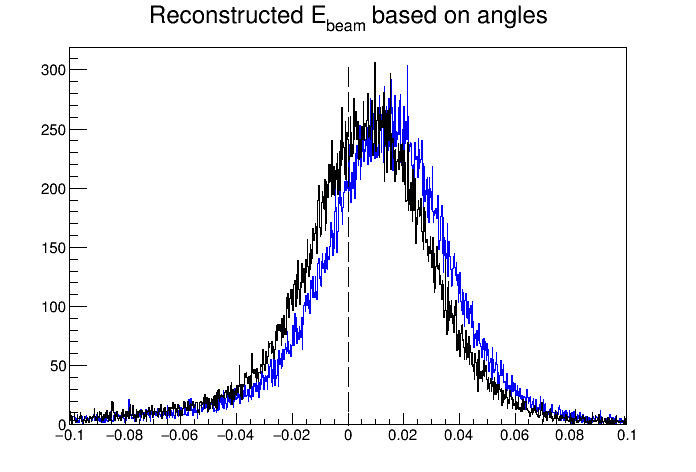
\includegraphics[width=12cm]{../report-H/delEnergy.png}\\
Beam energy reconstruction compared to what is measured. The black curve shows the distribution after applying the pointing corrections. The distributions improve by about 5.7 MeV. Ideally, one would want to look at the distribution with extended-target-rastered-beam corrections applied, but this requires to re-analyze the entire file, which takes quite a bit of time.
\end{center}

\begin{center}
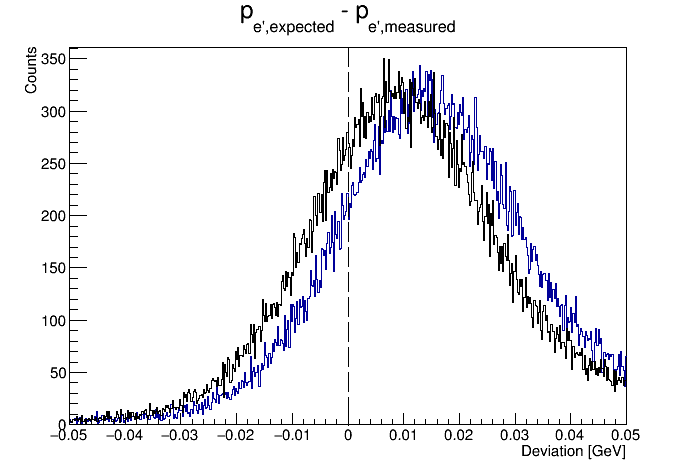
\includegraphics[width=13cm]{../report-H/delPe.png}\\
The black curve shows the distribution after applying the pointing corrections. Another source of error in these distributions is uncalibrated offsets of central momentum.
\end{center}

\begin{center}
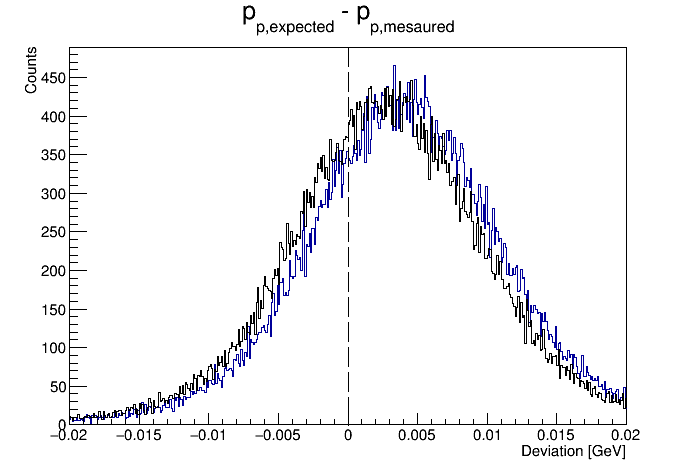
\includegraphics[width=13cm]{../report-H/delPp.png}\\
The black curve shows the distribution after applying the pointing corrections. Another source of error in these distributions is uncalibrated offsets of central momentum.
\end{center}

\begin{center}
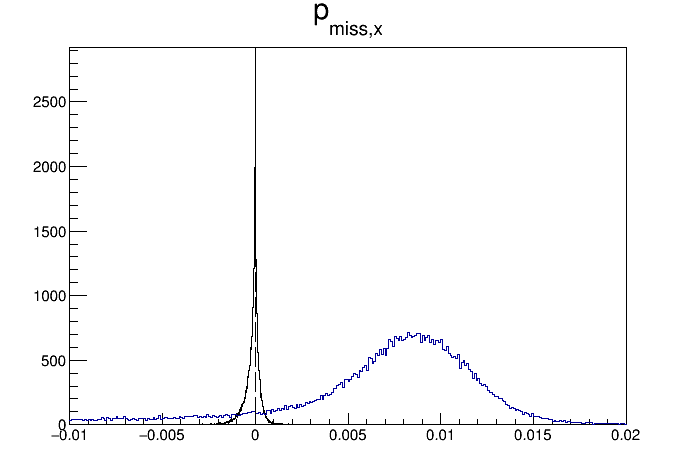
\includegraphics[width=13cm]{../report-H/delPmx.png}\\
The black curve shows the distribution after applying the pointing corrections. Another source of error in these distributions is uncalibrated offsets of central momentum.
\end{center}

\begin{center}
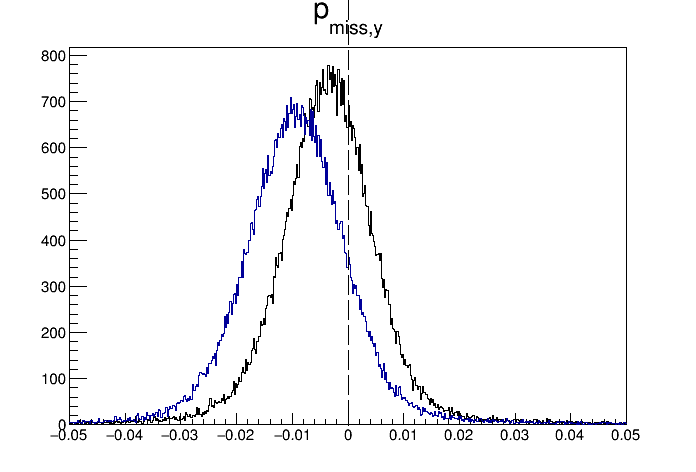
\includegraphics[width=13cm]{../report-H/delPmy.png}\\
The black curve shows the distribution after applying the pointing corrections. Another source of error in these distributions is uncalibrated offsets of central momentum.
\end{center}


\begin{center}
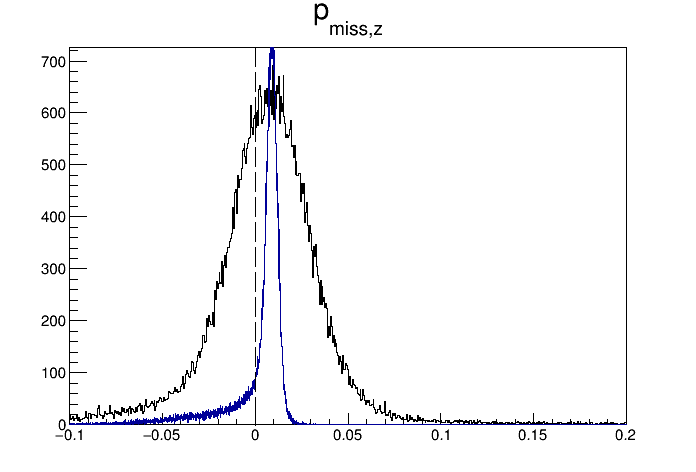
\includegraphics[width=13cm]{../report-H/delPmz.png}\\
The black curve shows the distribution after applying the pointing corrections. Another source of error in these distributions is uncalibrated offsets of central momentum. It's a bit strange this became so wide, perhaps it's because we are including energy of beam error? This is a bit familiar to the last plot in the hydrogen report.
\end{center}

\clearpage
\begin{thebibliography}{99}

\bibitem{}
Shout-out to Barak

\bibitem{nim}
J. Alcorn \textit{et al.}, Nucl. Inst. Meth. A \textbf{522}, 294, (2004); see also \url{hallaweb.jlab.org/equipment/Hall-A-NIM.pdf} 

\bibitem{techNote}
P. Ulmer, H. Ibrahim, Jefferson Lab Technical Notes JLAB-TN-00-024, (2000); see also \url{hallaweb.jlab.org/publications/Technotes/files/2000/00-024.pdf}

\bibitem{thesis}
F. Benmokhat, PhD thesis, Rutgers University, (2004); see also \url{https://misportal.jlab.org/ul/publications/view_pub.cfm?pub_id=5609}

\end{thebibliography}


%%%%%%%%%%%%%%%%%%%%%%%%%%%%%%%%%%%%%%%%%%%%%%%%%%%%%%%%%%%%%%%%%%%%%%%%%%%%%%%%%%%%%%%%%




\end{document}
